\section{Introducción}
\setcounter{sectiontotal}{3}

\begin{frame}
\frametitle{\pagetitle}
\framesubtitle{Descripción}
\begin{figure}
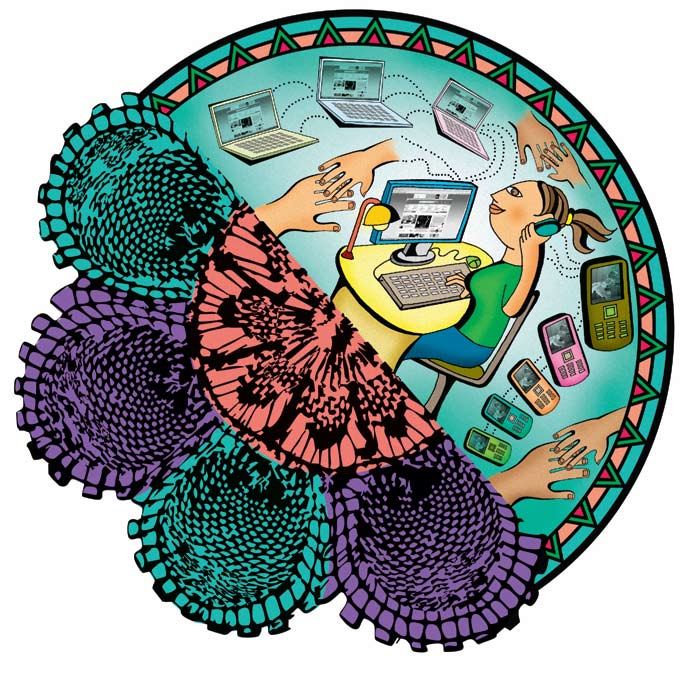
\includegraphics[scale=.3]{imagenes/nhanduti}
\end{figure}
\end{frame}

\begin{frame}
\frametitle{\pagetitle}
\framesubtitle{Objetivo general}
\begin{block}{Descripción}
\centering
Identificar y valorar los aspectos pedagógicos, de diseño, de implementación y
de evaluación que influyen a la creación de herramientas educativas que utilizan
las corrientes pedagógicas actuales apoyadas en las TIC, especialmente los
juegos serios.
\end{block}


\end{frame}

\begin{frame}
\frametitle{\pagetitle}
\framesubtitle{Objetivos específicos}

\small
\begin{enumerate}[<+->]

\item Proveer una visión actualizada de los fundamentos y estado del arte de las
    nuevas corrientes pedagógicas y su relación con las TIC.

\item Proveer una visión actualizada de los juegos serios, sus principales
    características y sus ventajas y desventajas como herramientas pedagógicas.

\item Identificar áreas de aplicación de los juegos serios, para determinar un
    contexto local factible para su aplicación.

\item Clasificar y seleccionar las herramientas tecnológicas disponibles para el
    desarrollo de soluciones que involucran a los juegos serios.

\item Contrastar en la práctica los conocimientos teóricos adquiridos a través
    del diseño e implementación de un juego serio.

\item Evaluar la solución propuesta para la obtención de datos que permitan
    identificar aspectos de diseño, desarrollo y evaluación a tener en cuenta
    para la creación de un juego serio.

\end{enumerate}

\end{frame}

